\documentclass[11pt]{article} %Type of document
\usepackage[english,]{babel} %Languages
\usepackage[T1]{fontenc} %Font Package
\usepackage{charter} %Font Type
\usepackage{geometry}
\geometry{letterpaper, portrait, margin=2cm}
\usepackage{graphicx} % Required for inserting images
\usepackage{url}
\usepackage{amsmath}
\graphicspath{{images/}} %configuring the graphicx package
\usepackage{parskip} % No Indent
\renewcommand{\baselinestretch}{1.5} % Line Spacing
\setlength{\parskip}{1em} % Pararaph Separation
\usepackage{pifont} % Itemize symbols
\renewcommand{\labelitemi}{\ding{111}} % Type of itemize symbol
\usepackage{hyperref} % hyperlink types
\hypersetup{
    colorlinks=true,
    linkcolor=blue,
    filecolor=magenta,      
    urlcolor=cyan,
    pdftitle={Overleaf Example},
    pdfpagemode=FullScreen,
    }

\title{Development of a Computational Framework for Simulating Spacecraft Fragmentation and Orbital Debris Population Dynamics}
\author{Juan Francisco Puerta Ibarra.}
\date{}

\begin{document}
\maketitle

\tableofcontents
\newpage

\begin{abstract}
The proposed research, within the Ph.D. in Engineering inside the Faculty of Engineering at Universidad de Antioquia, is to study the dynamics of spacecraft fragmentation~\cite{mains_impact_2021} and its impact on the sustainability of space exploration, orbital conjunction events and also to create some tools for space mission design, according to the growing problem of Low Earth Orbit (LEO) debris population. Numerical analysis, the database of space objects, and explosion and collision events are required to analyze and simulate the propagation of fragmentation debris from spacecraft and track not only the resulting objects but also create models to propagate backward and track the origin of the elements in actual orbit~\cite{letizia_analytical_2014}, as well as analyze the potential effects of different types of collisions and other events that can lead to fragmentation. This research will contribute to the development of more effective debris mitigation strategies and enable the continued exploration and utilization of different orbits in space exploration and utilization.
\end{abstract}

\section{Introduction}

The exploration of space has become an important subject for humanity, and specifically governments, and also private companies, with the commercialization of it in this new era of space industries. With increasing advancements in space technology, more spacecraft are being launched into orbit to collect data, generate revenue, and expand our understanding of the universe. However, the continued growth of the orbital population and, therefore, the creation of space debris resulting from the fragmentation of several of these assets poses a serious threat to the sustainability of space exploration, especially in orbits around Earth. 

In the span of less than a century since the commencement of activities in near-Earth orbits, a series of fragmentation incidents has transpired, leading to a notable upsurge in the population of potentially hazardous space debris~\cite{karacalioglu_impact_2016}. The scientific community is expressing particular apprehension regarding the persistent expansion of the small satellite market and the deployment of extensive constellations. Indeed, the likelihood of significant collisions among spacecraft is intricately tied to the burgeoning count of satellites in orbital realms, serving as a catalyst for potential cascade events that could impact the entirety of the near-Earth environment. Furthermore, historical occurrences such as the Cosmos-Iridium incident in 2009, 
where two satellites were circling the Earth with an approximate velocity of 7.5 km/s, colliding at a speed exceeding 10 km/s. The impact generated a range of space debris, ranging from sizable, substantial fragments to tiny dust particles. The resulting debris cloud poses a potential threat to satellites in close proximity, demonstrating that the resultant fragments extend beyond the altitudes directly implicated, reaching, and influencing neighboring orbits~\cite{wang_analysis_2010}.

Although effective strategies to avoid collisions and mitigation policies can minimize the risk of in-orbit collisions, there is a need to comprehend the mechanisms and dynamics involved in satellite and debris collisions and identify the key parameters influencing fragment generation. Presently, the NASA Standard Breakup Model (SBM) stands as the primary tool for predicting fragment distributions resulting from collision events. Based on the Impact Energy-to-Mass Ratio (EMR), this semi-empirical model utilizes the mass or momentum of the involved bodies as input parameters. However, due to its inherent simplicity, the NASA SBM lacks the ability to distinguish between events with the same specific energy, such as central versus glancing impacts~\cite{johnson_nasas_2001}.

This is where the focus of this proposed research, interest, and passion for astrodynamics and space sustainability analysis related to spacecraft breakups for space debris forensic analysis comes in.

\section{Theoretical Framework}

\subsection{Fundamentals of Space Debris}

Space debris encompasses defunct satellites, spent rocket stages, fragments from collisions, and other remnants of human space activities. It populates Earth's orbit, posing challenges to operational spacecraft and future space missions. Understanding the dynamics of space debris involves considering its types and the mechanisms leading to its creation. Space debris can be broadly categorized into two main types: large objects and small particles. Large objects include defunct satellites, spent rocket stages, and fragments from previous collisions. Small particles, often referred to as micrometeoroids or paint flecks, result from the continual erosion and fragmentation of larger objects due to natural forces in the space environment, orbital perturbations, and the upper atmosphere, among others.

As the quantity of artificial satellites and objects orbiting the Earth continues to rise as shown in Figure ~\ref{fig:typeobject}, the likelihood of collisions among these satellites also escalates. These collisions would result in the creation of orbiting fragments, each contributing to an increased probability of subsequent collisions. This sequence of events could lead to the expansion of a debris belt encircling Earth, drawing parallels with theories regarding the formation of asteroid belts. The flux of debris in such an Earth-orbiting belt might surpass the natural influx of meteoroids, thereby influencing the design considerations for future spacecraft. Using a mathematical model, predictions were made regarding the potential rate of formation for such a belt. Under specific circumstances, the initiation of this belt could commence within the current century and pose a notable challenge in the subsequent century. The presence of numerous undetected fragments resulting from spacecraft explosions could potentially shorten this time frame. However, the early adoption of specialized launch restrictions and operational protocols has the potential to substantially postpone the formation of the debris belt.

\begin{figure}
    \centering
    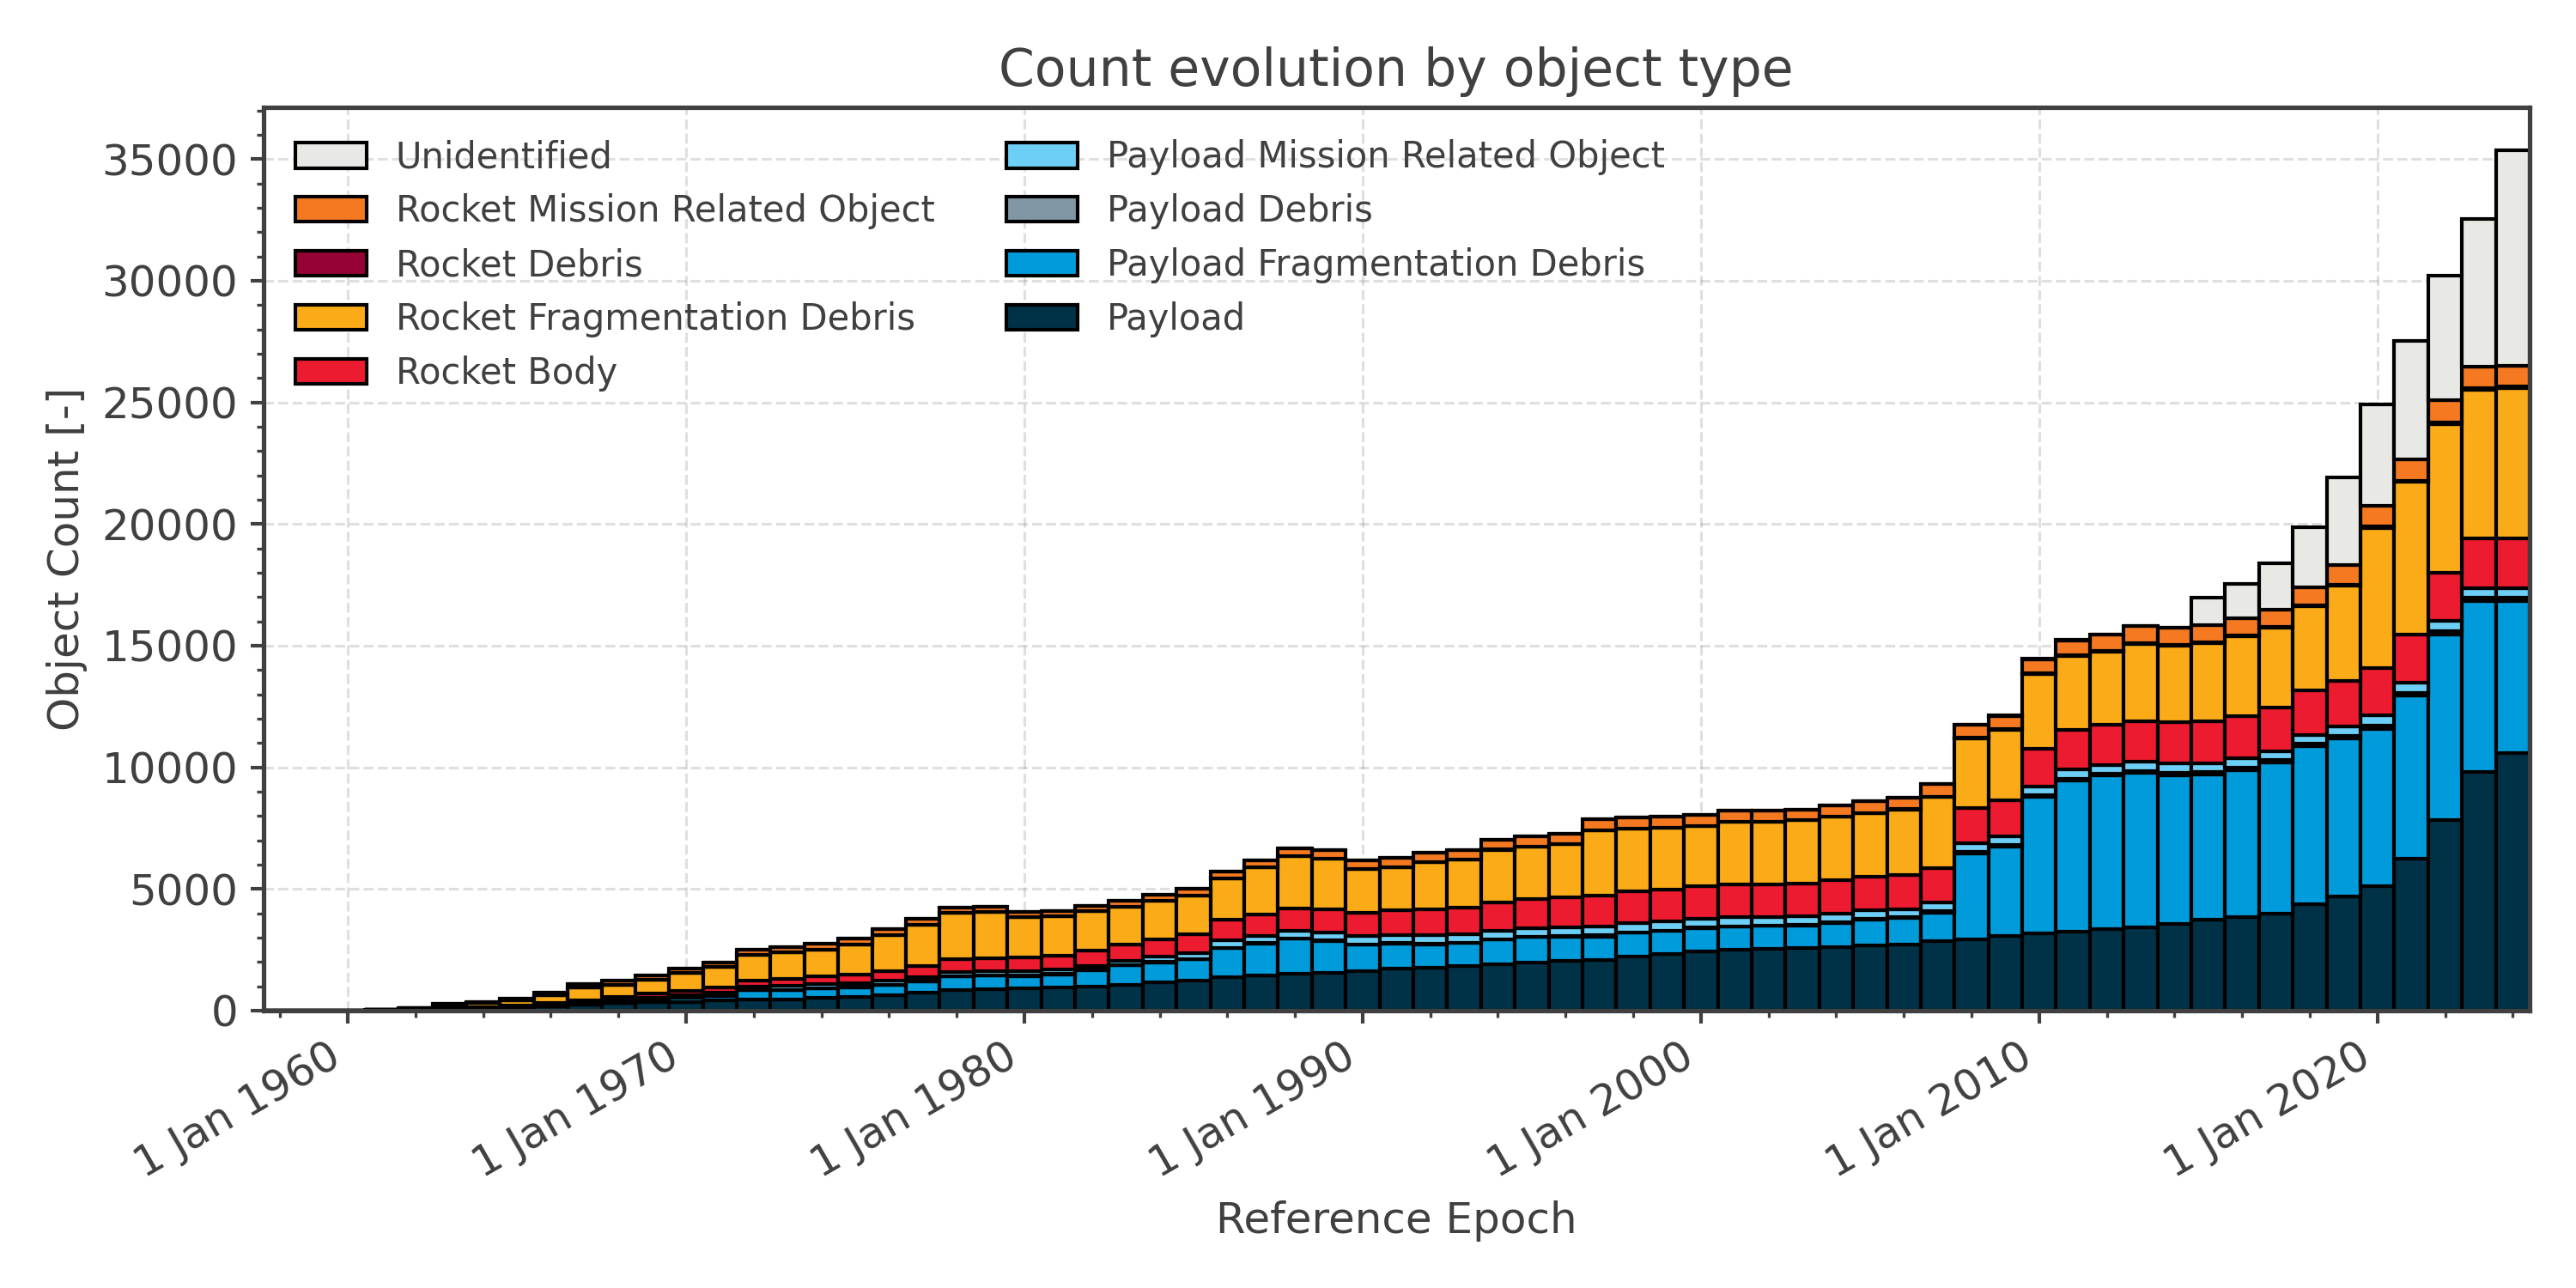
\includegraphics[width=1\linewidth]{allEvoTypeCnt.png}
    \caption{Evolution of the number of objects in geocentric orbit by object class. Source: Source: \href{https://sdup.esoc.esa.int/discosweb/statistics/}{Space Debris Environment Report issued by ESA's Space Debris Office, 2023}}
    \label{fig:typeobject}
\end{figure}

The concept known as the Kessler syndrome, initially theorized by Don Kessler and Burt Cour-Palais in 1978, has been a focal point in extensive global research. This syndrome, which revolves around the collision among space objects, is considered one of the most challenging aspects of managing orbital debris~\cite{kessler_collision_1978}. It has the potential to generate a substantial number of fragments per collision event, posing a significant threat. If the frequency of collisions surpasses the natural atmospheric cleansing process, a chain reaction may ensue, gradually but inevitably increasing the overall debris population in densely populated areas of space. This phenomenon has garnered widespread attention, leading to numerous publications, dedicated workshops, and special sessions during international congresses. Recent studies, focusing primarily on major fragmentations in 2007 and 2009, suggest that the Kessler syndrome has indeed been set in motion. The consensus emerging from these studies underscores the importance of adhering to internationally agreed-upon mitigation rules to sustain space activities in the long term. Active deorbiting measures, specifically targeting at least five large objects annually from the most densely populated orbital regions, are deemed necessary for effective mitigation and remediation efforts. Collective findings emphasize the imperative to implement strategies to preserve the sustainability of long-term space operations.~\cite{bonnal_active_2013}

The dynamics of spacecraft fragmentation for an object in space is a complex problem that involves multiple physical processes such as collisions, explosions, and gravitational interactions, and space weather must be included to characterize the problem correctly, due to the extreme operational conditions and mission design requirements. The fragmentation process can be modeled, in the first stage, using numerical integration techniques~\cite{isoletta_orbital_2021}, such as Runge-Kutta or Prince-Dormand, i.e., to obtain the state vector (position and velocity of space objects) or their orbital elements (semi-major axis, eccentricity, inclination, etc.) and then propagating its positional state in backward or forward direction, depending on the ephemerides of the event. One initial idea is to get the latest state vector (position and velocity coordinates in the Cartesian coordinate system) with their TLE (Two Line Elements) information, simulate it going backward, and find how the particles were ejected after the fragmentation event. Using computational analysis such as orbital propagators based on physics dynamics is the first step to understanding the equations and models ruling the phenomena. More advanced models are required since they involve not only the motion of the objects in space but also the fragmentation process in orbit.

\subsection{Conjunction of Objects in Space}

In the past decade, a combination of economic incentives and political objectives has accelerated space launches, contributing to a continuous growth in both active satellites and space debris. Consequently, satellite operators and space agencies globally have a keen interest in precisely assessing the risk of potential collisions and determining necessary collision avoidance maneuvers. Recognizing that unmitigated collision risks in the short term can lead to long-term environmental degradation, proactive measures are imperative.

As universally recognized within the Space Situational Awareness community, the frequency of conjunctions is anticipated to significantly increase in the future, primarily due to the proliferation of new megaconstellations, small satellites, and other payloads. The introduction of these novel payloads is expected to exert a considerable impact on the space environment, manifesting in heightened collision risks, atmospheric pollution, and surface impacts. The increasing number of operational satellites accentuates the relevance of collision avoidance strategies, particularly in scenarios involving two active satellites. In such cases, the assessment of conjunctions and maneuvers necessitates a distinct approach compared to situations involving an active satellite and space debris, where only the active satellite is capable of executing maneuvers.~\cite{oltrogge_collision_2016}

\subsection{Space Debris Fragmentation}

Since 1961, more than 80 incidents of satellite fragmentation have been identified. These events account for one-third of all human-made objects in space documented since the launch of Sputnik 1 and constitute half of the satellites currently orbiting Earth. The two recognized causes of artificial satellite break-ups are accidental occurrences, often related to propulsion malfunctions, and deliberate actions, such as military-related onboard explosions. However, the reasons behind fifty percent of satellite breakdowns remain unknown, although in Figure ~\ref{fig:enter-label} the unknown causes are more likely to be predominant. The continual growth in the population of near-Earth space debris raises valid concerns regarding the increasing likelihood of collisions between satellites. The constraints of ground-based radars imply that the actual number of Earth-orbiting satellites could be significantly higher than officially registered. Recent laboratory experiments indicate that a substantial number of potentially hazardous fragments could be released during hyper-velocity collisions in space.~\cite{johnson_history_1985}

The effects of spacecraft fragmentation on space sustainability can be analyzed using various metrics, such as the creation of new debris, the risk of collision with operational spacecraft, and the potential impact on scientific observations. Mitigation of space debris can be achieved through various methods, such as active debris removal and collision avoidance techniques. The effectiveness of these methods can be assessed through more precise numerical simulations and statistical analyses.

\begin{figure}
    \centering
    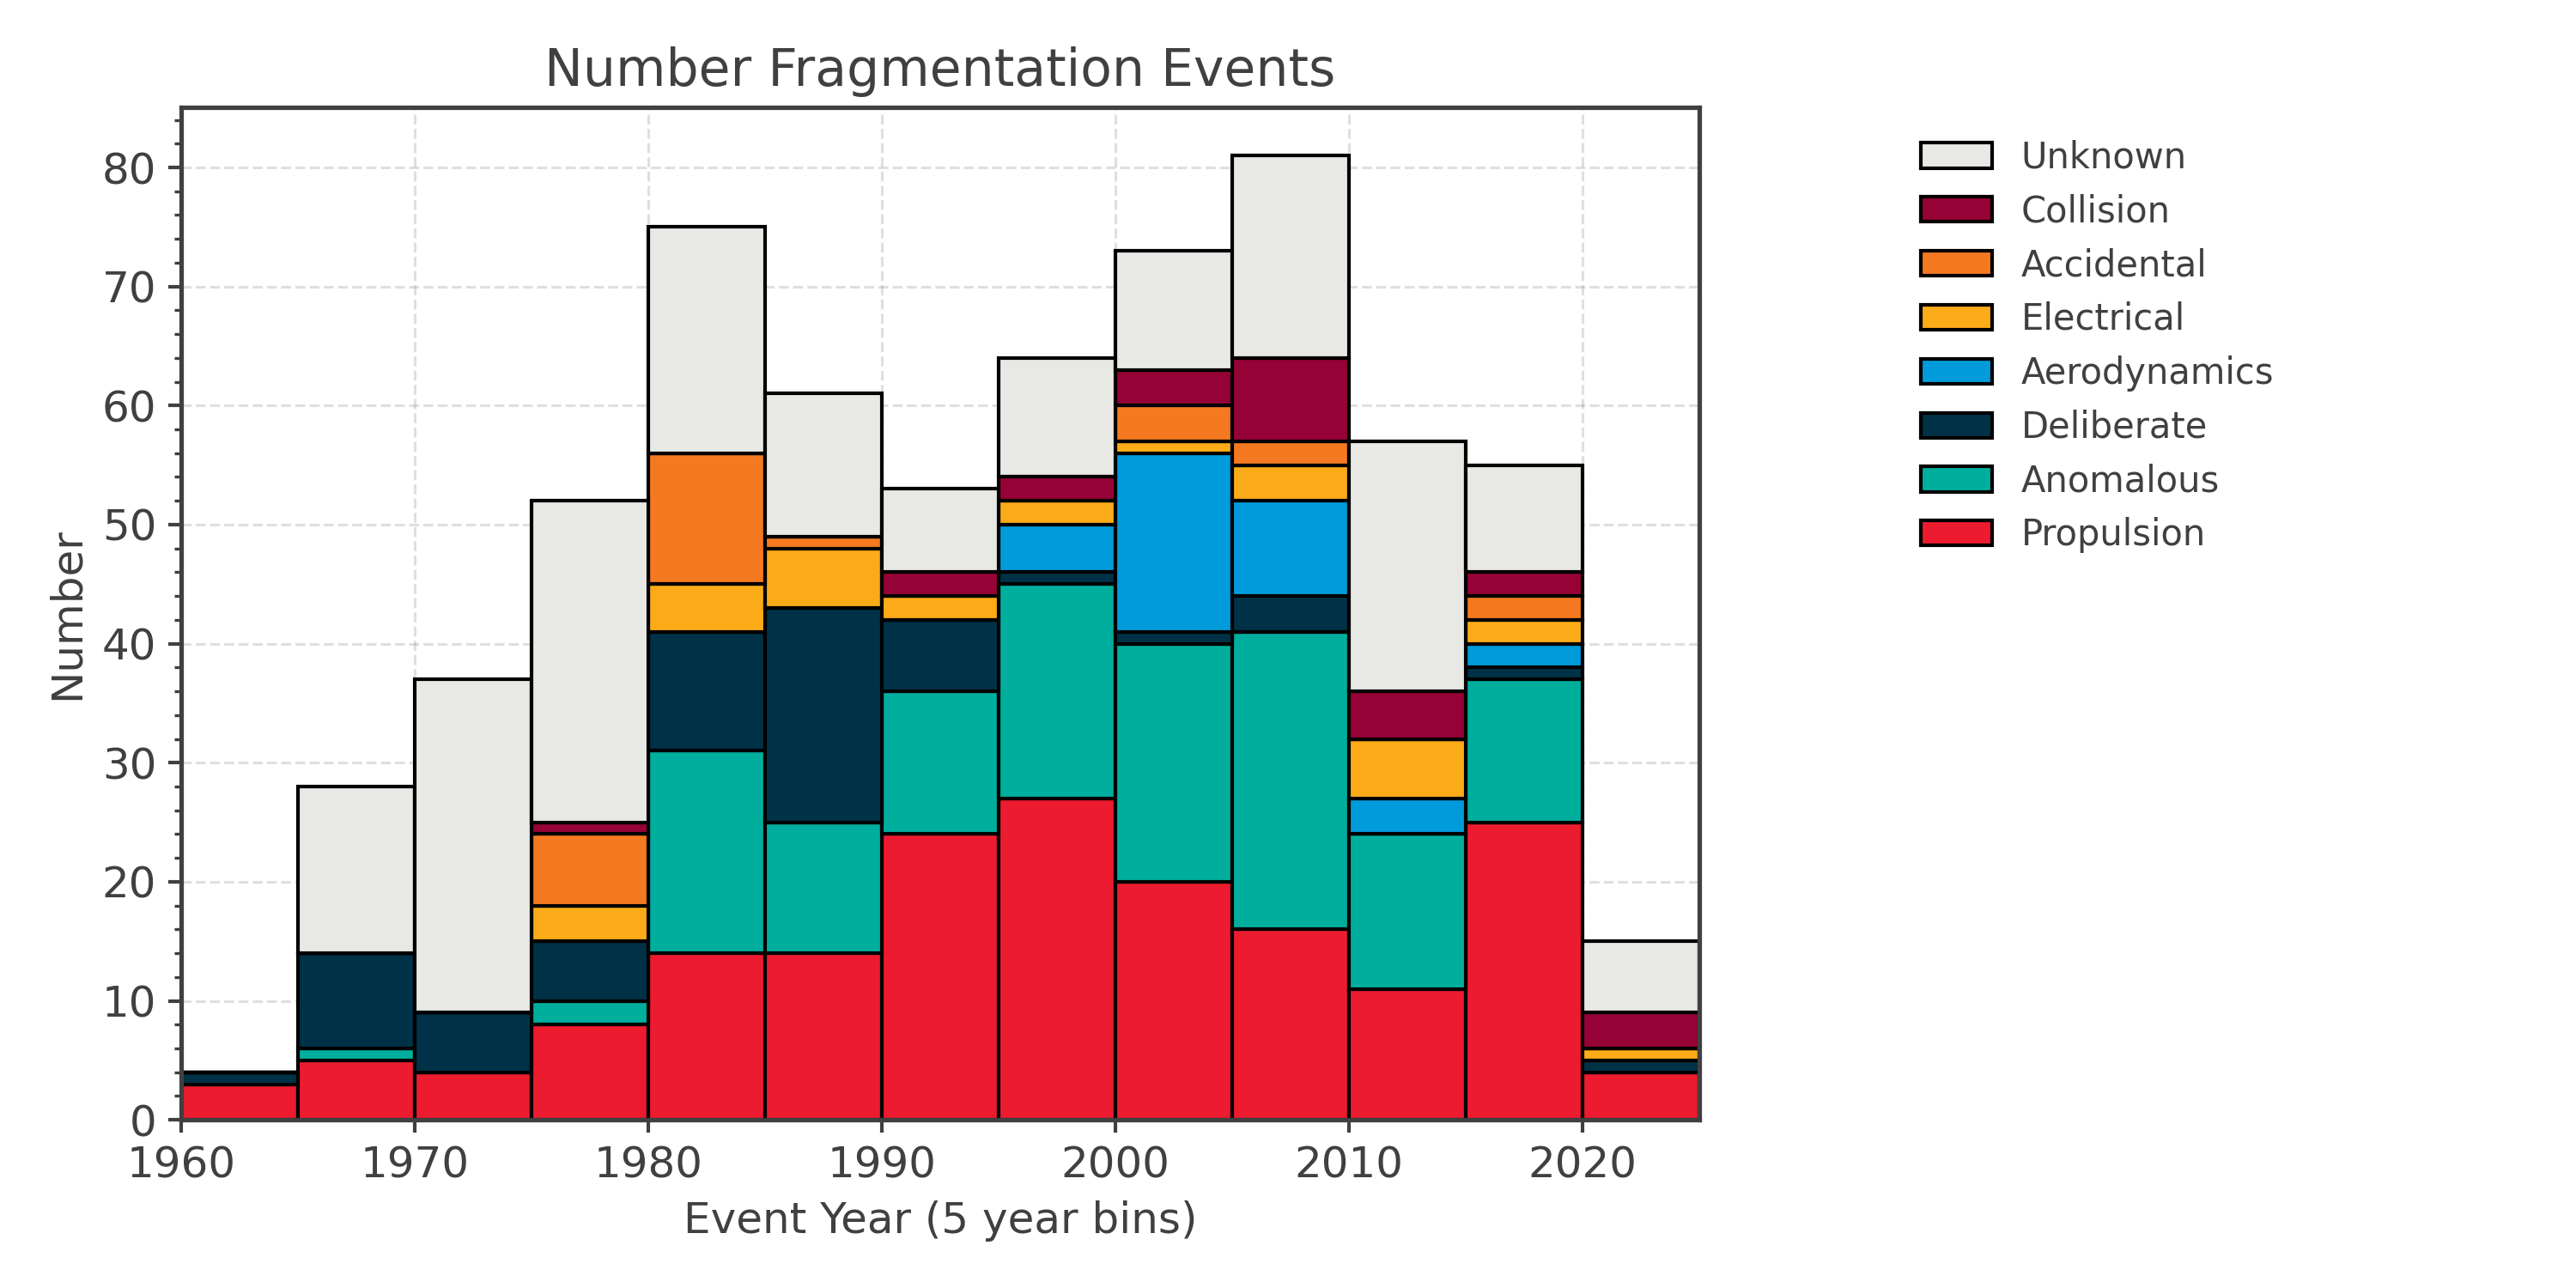
\includegraphics[width=1\linewidth]{eventCausesPerEY_abs.png}
    \caption{Historical trend of fragmentation events per event cause. The last bin covers until the year 2022. Source: \href{https://sdup.esoc.esa.int/discosweb/statistics/}{Space Debris Environment Report issued by ESA's Space Debris Office, 2023}}
    \label{fig:enter-label}
\end{figure}

\subsection{Causes of Space Debris Fragmentation}

Understanding the causes and effects of space debris fragmentation is extremely important to determine the behavior, modeling, and development of new approaches and computational tools for appropriate analysis. Furthermore, understanding these factors is crucial to modeling events more precisely and devising futuristic scenarios based on the initial data. Several primary factors contribute to the fragmentation of space debris.

On average, there have been 11.2 instances of non-deliberate fragmentations annually in the space environment over the past two decades. While this figure remains relatively consistent, the impact of each event varies. When considering the lifespan of the generated fragments, this number notably decreases to 2.5 per year, and further drops to 0.4 per year when systematic and unexplained events are excluded from the analysis. This suggests that non-collisional events, which can have a substantial environmental impact, persist, potentially attributed to the reuse of a design with known issues. In particular, fragmentations other than collisions currently represent the primary source of space debris. The escalating launch traffic and the enduring nature of space debris events in the low Earth orbit contribute to a considerable conjunction risk in the most congested Earth orbits.~\cite{european_space_agency_space_nodate}

\subsubsection{Collisions}
High-velocity impacts between space debris and operational satellites or other assets in orbit occur at high relative velocities, generating smaller fragments in the process with a large amount of energy released. These collisions have been studied, and their implications are documented, but the amount of information is still not enough for a more profound analysis.

Cascading collisions can result from these initial collisions, leading to further break-up events and exacerbating the debris problem. The cascade effect is a significant concern in the context of space debris dynamics and mitigation efforts, based on the initial concept explained by Don Kessler in 1978. The primary idea behind this concept is that a single collision between two space objects can create a cloud of smaller debris fragments. These fragments, in turn, pose a significant risk to other operational satellites and space assets, potentially leading to additional collisions and more fragmentations.~\cite{kessler_environment_1985}

\subsubsection{Explosions}
Explosive decompression can occur due to explosions of defunct satellites, spent rocket stages, or malfunctioning components. These events can be due to various factors, including residual propellants, batteries, or other hazardous materials within the system, mostly after some years of operations in space. The outcome is often the disintegration of the original object into smaller fragments.

When an explosion event occurs, it can generate a cloud of smaller fragments. The sizes of these fragments can vary widely, ranging from large pieces to tiny shards and even micrometer-sized particles. The number of fragments created depends on the magnitude of the explosion, the materials involved, and the specific circumstances of the event. These fragments are then released into various orbits around the Earth.

Accurate modeling of space debris from explosion events is essential for space situational awareness and collision avoidance. As discussed above, mathematical models and simulations are used to predict the trajectories and behavior of these fragments. However, the sheer number of debris pieces and the complex dynamics of their orbits make this a challenging task.

\subsubsection{Natural Forces}
Space debris is subject to natural forces, including micro-meteoroid impacts. These impacts gradually erode and fragment objects over time, contributing to the overall fragmentation of space debris. The impact of natural forces is a critical aspect in understanding the long-term dynamics of space debris. Micrometeoroids, tiny particles present in space, can collide with space debris fragments, leading to surface erosion and potential fragmentation. These impacts can gradually degrade the structural integrity of debris objects, causing them to break into smaller pieces or generating cracks and fissures.

Orbital fragments, once released into the Earth's orbit, are subjected to various natural forces that contribute to their evolution and behavior over time. These natural forces, originating from the space environment itself, can impact the dynamics and characteristics of space debris, influencing their trajectories and potential collision risks. By being in orbit, gravitational interactions with additional celestial bodies besides Earth, such as the Moon or the Sun, can perturb the orbits of space debris fragments. These gravitational forces can cause variations in the orbital parameters of residual objects, leading to changes in their positions, velocities, and orbital planes. Over time, these perturbations can result in alterations to the distribution and density of debris fragments within different orbital regions.

Space weather, primarily created by the Sun, is an important factor to consider, since solar radiation exerts pressure on these objects, especially those with larger surface areas. This pressure can influence the orbits of debris objects, leading to changes in their trajectories over time. These forces, while relatively weak, can gradually alter the paths of debris fragments, potentially increasing the risk of collisions with other space assets. Moreover, the Earth's environment from the atmosphere creates drag, leading to a gradual decrease in their orbital altitudes. This drag force results from the interaction between elements in low-earth orbit and the Earth's atmosphere, causing their positions to decay over time. As their orbits decay, the debris fragments may re-enter the Earth's atmosphere, leading to their eventual incineration or impact on the planet's surface.

\subsubsection{Deliberate Actions}
Deliberate actions in space, such as anti-satellite (ASAT) tests, significantly contribute to space debris fragmentation. These actions involve the intentional destruction of a satellite or space object, often for military or scientific purposes. The primary reason for these activities leading to the fragmentation of space debris is the violent nature of the destruction, from a kinetic point of view of the analysis, which generates a large number of debris fragments. Certain space missions intentionally fragment objects in orbit, often for scientific research or military purposes. The Fengyun 1C event from an ASAT (Anti-Satellite Weapons Test) made by China in 2007, is a notable example of the impact of the test in the space environment in LEO. These deliberate actions can lead to the generation of additional debris fragments, contributing to the already complex space debris environment.

 In an ASAT test, a satellite or space object is typically destroyed using a kinetic device, usually from a missile launched from the surface of the Earth or by a military aircraft. When the impact process is produced, it causes the target satellite to rapidly decompress. This explosive decompression results in the disintegration of the satellite into numerous smaller pieces. These fragments can vary in size and can include structural components, electronics, and other satellite materials. Fragments produced during an ASAT test are ejected from the site of the explosion at high relative velocities, often exceeding the speeds typical for space debris in orbit. These high velocities can increase the kinetic energy of the fragments, making them potentially more dangerous and more prone to damage in the event of a collision.~\cite{sorge_orbital_2008}

\subsection{Tracking and Cataloging}
Tracking and cataloging space debris objects is a challenging but vital task for space debris fragmentation analysis. The difficulty arises from the vast number of objects in orbit, their small sizes, varying orbits, and the need for continuous monitoring. However, the importance of this endeavor cannot be overstated, as it forms the foundation for understanding the behavior and risks associated with space debris.

Space is crowded with objects, including operational satellites, defunct spacecraft, spent rocket stages, and various fragments. Some of these objects are as small as paint chips, making them challenging to track. The task is further complicated by the diversity of orbits they occupy, from low Earth orbit (LEO) to geosynchronous orbit (GEO). Tracking space debris is akin to finding and monitoring thousands of moving targets in a vast, dynamic, and three-dimensional environment. Accurate tracking and cataloging are essential for understanding the distribution of space debris in Earth's orbit. The data gathered through tracking systems helps identify regions with higher debris density and areas with a greater risk of collisions. This knowledge is critical for spacecraft operators to plan and execute maneuvers to avoid potential collisions.~\cite{watson_optical_2019}

The process of tracking debris in orbit enables the prediction of close approaches and potential collisions between those elements and operational satellites. Timely warnings of such events allow satellite operators to adjust orbits or take other preventive measures to protect their assets. This is crucial for maintaining the safety and functionality of operational satellites.~\cite{noauthor_space_nodate}

\subsection{Modeling Space Debris Fragmentation}

Modeling space debris and space fragmentation is a complex task that involves understanding, predicting, and mitigating the risks posed by objects in Earth's orbit. Challenges in this field are multifaceted, stemming from the abundance of debris, evolving debris characteristics, and the need for robust analytical tools. One of the primary challenges in modeling space debris is the sheer number of objects. Thousands of satellites, rocket stages, and fragments of various sizes and materials orbit Earth. This population is constantly evolving due to new satellite deployments, collisions, breakups, and other space activities. The size and distribution of space debris fragments vary widely.~\cite{noauthor_debris_nodate}

The movement of space debris is governed by complex gravitational interactions, radiation pressure, and non-gravitational forces. The accuracy of debris models depends on the quality and completeness of the available data. Gaps in the catalog of space objects, especially small fragments, pose a significant challenge due to the inability of space-tracking networks to detect objects smaller than 10 cm in diameter. Therefore, there are different approaches for modeling orbital debris to be considered.

\subsubsection{Analytical models.}

Analytical models are mathematical representations of the behavior of space debris based on simplified physical principles and assumptions. They are valuable for gaining quick insights into specific scenarios. Certain fragmentation incidents yield only a limited number of objects and may rapidly decay as a result of atmospheric drag. However, in most cases, a substantial number of fragments are produced, which significantly increases the risk of collisions that satellites encounter throughout their operational lifetime. As part of ongoing efforts to implement debris mitigation measures, space agencies and academic institutions are consistently working on the development of models and software. These tools are designed to analyze the space environment, estimate the likelihood of collisions between cataloged space objects, and forecast the future expansion of the debris population.

An integral element within models depicting the evolution of orbital debris environments is the satellite breakup model. Widely acknowledged as the global standard, the NASA standard breakup model (SBM) has been incorporated into both EVOLVE 4.0 and later versions like LEGEND~\cite{johnson_nasas_2001}. This model yields three essential outcomes: the distribution of fragment sizes, the area-to-mass ratio (A/M), and the distribution of relative velocities ($\Delta{v}$). These distributions have been derived from a diverse range of data sources, encompassing intentional hypervelocity collisions in low Earth Orbit (LEO), impacts on Earth's surface, tests involving the explosion of upper stages, and a comprehensive compilation of historical orbital data (e.g., Two-Line Element sets) concerning debris resulting from explosions and collisions.

\subsubsection{Numerical models.}

Numerical space debris models are advanced computational tools that simulate the motion and evolution of space debris in a highly accurate manner. These models rely on numerical integration techniques to solve the equations of motion for a large number of individual debris objects. They take into account various forces and perturbations that affect space debris, providing detailed predictions of object positions and velocities over time. They typically use high-precision numerical integration methods, such as the Runge-Kutta method, to calculate the position and velocity of space debris objects in discrete time steps. These methods ensure accurate trajectory predictions.

This concept of a more robust computational model considers various perturbations that influence orbital motion, including gravitational forces from Earth, the Moon, the Sun, and other celestial bodies. These models also account for non-gravitational effects like atmospheric drag and solar radiation pressure. In theory, they can simulate collisions between space debris objects and track the resulting fragments with the ability to calculate the characteristics of fragments, such as mass, size, and velocity, which are vital for assessing collision risks and estimating the growth of the debris population. These types of models are resource-demanding and require high-performance clusters for their calculations. 

As a practical example, the NORAD Two-Line Element Set (TLE) format is often used to represent the orbital elements of space debris objects. Numerical models process TLE data to generate precise orbit predictions. These models are employed by organizations like NORAD (North American Aerospace Defense Command) and ESA (European Space Agency) to manage space debris.~\cite{vallado_two-line_2012}

\section{Background and literature review.}

There are more than 35,000 space debris objects detected, 10 cm or more in diameter,  since the beginning of human space exploration from the end of the 1950s until the end of 2020s. (Citation Samuel Diserens). Since the first discussion and analysis of the impact of human-made space objects by Don Kessler (Kessler citation), the number of these elements in orbit has increased and noncataloged objects present a dangerous threat~\cite{diserens_newspace_2020,kessler_environment_1985}.  Between the sizes of 10 cms and 5 cms, a satellite can be destroyed and if the debris has a smaller scale, like 1 mm, it can create perturbations on any operating spacecraft, from structure failure to attitude changes.

Fragmentation events can be considered as explosions and collisions in orbit. The population created is measured and characterized from earth observations made by radars and telescopes. The number of events has been increasing to around five per year ~\cite{horstmann_survey_2018}. Another challenge from the registered events is to analyze and review these known events. The amount of information for a computational model to have a general usage and precision is still small and basically is conceived to have a statistical approach. Modeling a fragmentation event, from a pure physics perspective, is extremely challenging because of the computation resources required and the time to obtain a solution. Therefore, creating new scenarios for fragmentation events based on simulation models can be difficult.

\subsection{Debris and fragmentation modeling.}

Small objects in debris simulation models require a simplified but elegant and accurate approach to describe the evolution of a cloud of objects in space, making the analysis of a collision or explosive event a very demanding process. Analytical models (cite) describing the behavior of artifacts in orbit have been proposed mainly for small-duration events where the forces can be represented by Hamiltonian mechanics ~\cite{letizia_continuity_2014}. The analysis of long-term population where space debris density is high was presented by McInnes in 1993, by considering the population in Low Earth Orbit as a fluid with continuous properties. This approach has been complemented by Nazarenko, who describes the progression of the number of objects in LEO based on the continuity equation with his own development ~\cite{letizia_multidimensional_2016}:

$$
\frac{\partial N_j}{\partial t}=-W_j\frac{\partial N_j}{\partial r}-N_j\frac{\partial W_j}{\partial r}+\dot{N_j} 
$$

where $N_j(r,t)$ is the number of elements in the $j^{th}$ bin regarding size, perigee altitude (rp), eccentricity (e), inclination (i), and ballistic coefficient. $W_j$ is the radial velocity of the objects and $\dot{N_j}$ is the rate of variation in the number of objects based on external causes. Based on the equation presented, the discussion is about the advantage of having a statistical model based on density compared to a deterministic model whose results are obtained by inputs and a set of equations describing the system, without randomness or uncertainty.

To create a precise model for space debris, it is essential to not only account for recent occurrences but also maintain a comprehensive historical record of in-orbit fragmentations on an ongoing basis. Presently, there are 261 recognized fragmentation events, with each one treated as a distinct incident in the modeling process. While there are some additional events labeled unknown anomalies, they are excluded from the fragmentation modeling phase. All the acknowledged events are classified as either explosions or (non-)catastrophic collisions, with detailed data on event characteristics such as mass and collision velocity. Of these 261 events, 247 are classified as explosions, making up approximately 95\% of the total. The remaining 14 events are designated as confirmed, for example, the Fengyun-1C Anti-Satellite Test, and assumed collisions. However, when examining the overall amount of tracked debris by the Space Surveillance Network (SSN), there are twice as many fragments resulting from explosions compared to those from collisions. Figure 1 shows the number of fragmentations over the last 60 years ~\cite{horstmann_survey_2018}. 

\begin{figure}
    \centering
    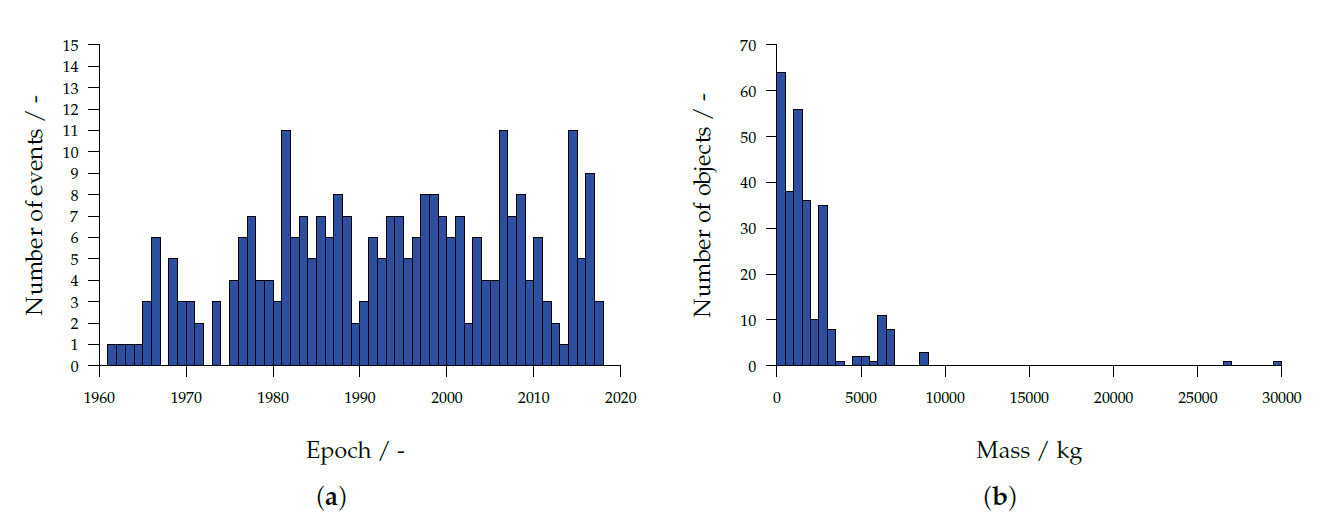
\includegraphics[width=1\linewidth]{Fig1.png}
    \caption{Assessment of the historical record of breakup incidents, including (a) the yearly count of in-orbit breakups, and (b) statistical data in the form of a histogram regarding the distribution of objects per fragmentation mass.}
    \label{fig:breakupincident}
\end{figure}

The average annual count of fragmentations is 4.9 (with a standard deviation of 2.8), and there is no observable trend of decline or significant alteration. However, there was a slight reduction in fragmentations over a three-year period following the implementation of the Inter-Agency Space Debris Coordination Committee (IADC) with its Space Debris Mitigation Guidelines in 2010. Figure 1b illustrates the examination of the fragmented mass over the years, highlighting that most of the objects that underwent fragmentation had a mass of less than 500 kg. On the opposite end of the spectrum in the histogram, there are two instances featuring a fragmentation mass of 26,000 kg and 30,000 kg. These occurrences date back to the late 1960s during the Apollo program; however, owing to their low orbital altitudes of below 300 km, nearly all fragments re-entered Earth's atmosphere, thereby making minimal long-term contributions to the space debris environment.

In recent times, the space sector has witnessed a notable phase of growth and transformation, characterized by the emergence of a burgeoning startup culture, often referred to as "NewSpace" or "the new space era". This shift is commonly linked to an amplified engagement of private investors and a change in priorities, diverging from the conventional practices of government and military-industrial entities. According to reports from Bryce Space and Technology, there has been a remarkable over twelve-fold rise in the annual average of investors in the space domain since the year 2000 ~\cite{diserens_newspace_2020}.

The phenomenon of fragmentation has been recognized as a critically significant aspect to focus on, and it's especially collisions that are anticipated to increasingly contribute to the generation of new space debris in the future setting. In the broader scope of creating models for the debris environment, understanding the mechanisms by which objects undergo fragmentation is vital. This comprehension not only helps in estimating the number of new objects introduced into the environment but also provides insights into their essential attributes, such as size, mass, and relative velocity of the parent body.

Among the existing range of debris models, nearly all of them predominantly rely on the NASA standard break-up model version 4.0, making it a subject of particular interest for further exploration. A notable exception to this trend is the Aerospace Corporation's ADEPT model, which employs an in-house tool called IMPACT. In the NASA model, first introduced in 2000, the process of generating debris fragments is based on the size or characteristic length ($L_c$) as the primary variable ~\cite{jenkins_strathcube_2021}. This characteristic length is then used to determine the mass, AMR (Area-to-Mass Ratio), and ejection velocity of the fragments. The distribution of fragments concerning their characteristic length ($L_c$) is outlined as follows:

$$
N(L_C) = \begin{cases} 
            6 S L_c^{-1.6}, & \textit{}{if } \textit{}{Explosion}\\
            0.1 M_e^{0.75} L_c^{-1.71}, & \textit{}{if } \textit{}{Collision}
\end{cases}
$$

The power law equation for explosions, which was derived from observations of fragments resulting from the explosion of various rocket bodies, is anticipated to apply to upper stages with masses ranging from 600 kg to 1,000 kg. For explosions originating from other sources, such as battery-related incidents or from different types of spacecraft, a type-dependent scaling factor, denoted "S," is chosen, typically falling within the range of 0.1 to 1.

In the event of a collision, the mass that's ejected, denoted as $M_e$, is determined using the following equation. This equation takes into account the masses of both the target object ($M_t$) and the projectile object ($M_p$), as well as the relative velocity ($v_{rel}$) between these two objects at the moment of impact.

$$
M_e= \begin{cases}
    M_t + M_p, & \textit{if } \textit{}{Catastrophic} \\
    M_p\left( \frac{v_{rel}}{1000} \right)^2, & \textit{if } \textit{}{Non-Catastrophic}
\end{cases}
$$

A catastrophic collision is characterized by the impacter's kinetic energy exceeding 40 joules per gram of the target mass. This equation governing collisions was formulated based on ground-based hypervelocity tests, like the SOCIT test series and the Solwind P-78 anti-satellite test, as on-orbit examples were lacking. The model's fundamental assumption is that all collisions will entail the complete involvement of each object's body. This model does not consider spacecraft that consist of multiple interconnected structures, including components like gravity gradient booms or deployed solar panels, which can impact the collision dynamics.

In the realm of space debris generation, historical trends have primarily revolved around spacecraft fragmentation. This process has been responsible for 65\% of the growth in the catalog of tracked objects since 2008 and constitutes 53\% of the total catalog, as indicated in NASA's "History of On-Orbit Satellite Fragmentations," 15th edition ~\cite{anz-meador_assessment_2004}. Of the 242 satellites believed to have experienced breakups since 1957, accidental collisions between objects account for only 2. 5\% of these incidents, compared to propulsion-based explosions, which account for 44.2\% of the events. Nonetheless, despite their lower frequency in absolute numbers, accidental collisions play a more substantial role in the cataloged debris, contributing to 11.6\% of the total. This underscores the notion that collision events, though infrequent, wield greater significance in shaping the overall development of the debris environment.

\section{Objectives.}

Design a general methodology for the analysis and simulation of space debris objects for fragmentation scenarios in orbit to study how space sustainability and population are affected.

\subsection{Specific Objectives.}
\begin{itemize}
    \item Develop an orbital propagator model, for energy conservation with the required perturbations, for an efficient simulation of the motion of space objects to preserve important properties of the system going forward and backward in time.
    \item Create an analytical, simple, and accurate model for the fragmentation events in space based on the initial conditions of the objects to study.
    \item Enable the model to predict the future orbits of both intact objects and debris fragments. This should include the ability to assess the evolution of the debris cloud resulting from fragmentation events.
    \item Develop a framework to conduct scenario-based analyses, such as the impact of mitigation measures on future debris growth, the assessment of debris populations in specific orbital regions, and the implications of different space missions.
    \item Perform sensitivity studies to evaluate how changes in model parameters, such as uncertainties in debris characteristics, affect fragmentation event outcomes and space debris evolution.
    \item Develop a user-friendly interface to facilitate the use of the model by space debris experts and agencies. This interface should allow users to input scenarios, view results, and conduct analyses efficiently to represent the simulated fragmentation events and their consequences.
    \item Ensure that the methodology complies with international guidelines and standards for space debris modeling and analysis.
\end{itemize}

\bibliography{references.bib}
\bibliographystyle{IEEEtran} %apalike

\end{document}